\section{Visualisations}
\begin{figure}\centering
    \incfig[]{ITAP}
    \caption{}
    \label{fig:ITAP}
\end{figure}

\begin{figure}\centering
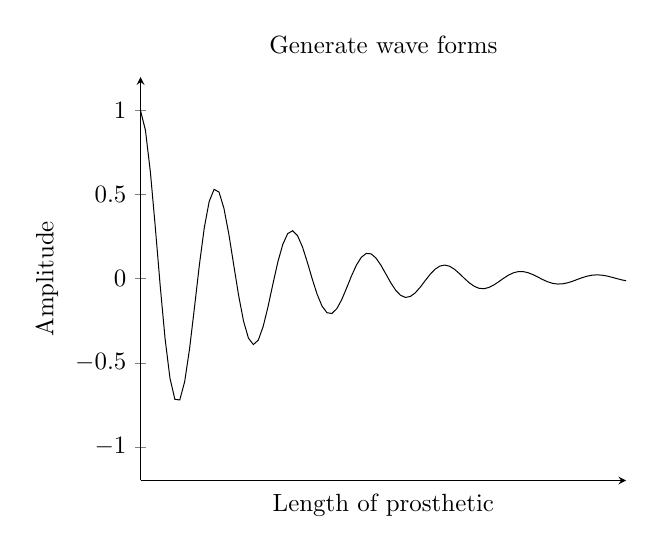
\begin{tikzpicture}[scale=0.9]
    \begin{axis}[
        xlabel = Length of prosthetic, ylabel = Amplitude, title = Generate wave forms,
        domain=0:40, xtick=\empty,
        samples=100,
        axis lines = left, ymax=1.2, ymin=-1.2
        ]
        \addplot[] {cos(deg(x))*exp(-0.1*x)};
    \end{axis}
\end{tikzpicture}
\end{figure}
\begin{figure}\centering
    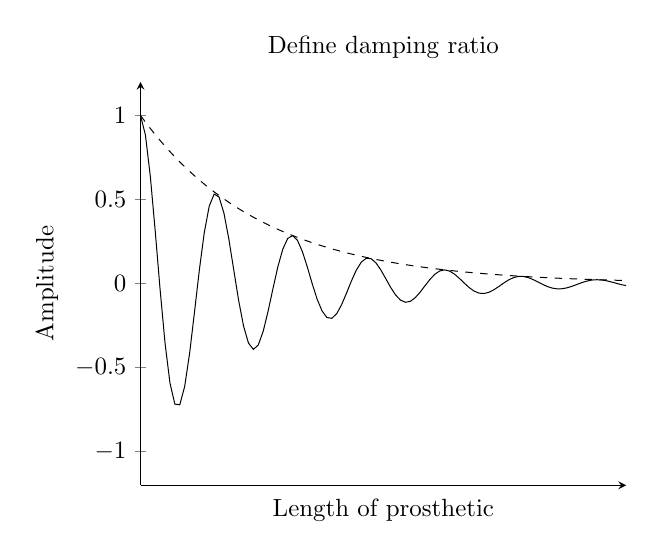
\begin{tikzpicture}[scale=0.9]
        \begin{axis}[
            xlabel = Length of prosthetic, ylabel = Amplitude, title = Define damping ratio,
            domain=0:40,xtick=\empty,
            samples=100,
            axis lines = left, ymax=1.2, ymin=-1.2
            ]
            \addplot[] {cos(deg(x))*exp(-0.1*x)};
            \addplot[dashed] {exp(-0.1*x)};
        \end{axis}
\end{tikzpicture}
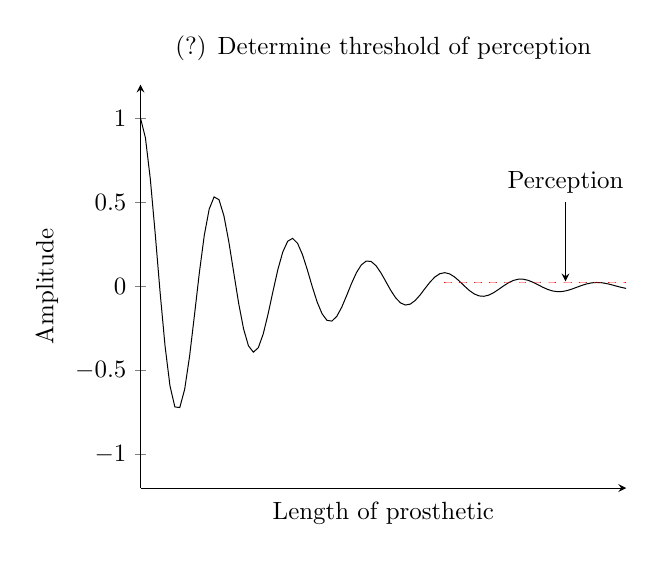
\begin{tikzpicture}[scale=0.9]
    \begin{axis}[
        xlabel = Length of prosthetic, ylabel = Amplitude, title = (?) Determine threshold of perception,
        domain=0:40,
        samples=100,xtick=\empty,
        axis lines = left, ymax=1.2, ymin=-1.2
        ]
        \addplot[] {cos(deg(x))*exp(-0.1*x)};
        \addplot[dashed, red, domain=25:40] {0.02};
        \draw[-stealth] (axis cs: 35,0.5) node[above]{Perception}-- (axis cs: 35,0.03);
    \end{axis}
\end{tikzpicture}
\end{figure}
